\subsection{Actuator}

\begin{wrapfigure}{r}{0.4 \textwidth}
    \centering
    \includesvg[pretex=\tiny, width = 0.35 \textwidth]{Gimbaled_thrust_diagram}
    \caption{The gimbal rotates the thrust force in order to impart a torque and a horizontal force~\cite{NASATVC}.}
\end{wrapfigure}
%\begin{wrapfigure}{l}{0.1\textwidth}
%    \centering
%    \includesvg[width = 0.1 \textwidth]{RCS}
%    \caption{\cite{Kehl2015}}
%\end{wrapfigure}
There has been previous success~\cite{BPS} in controlling \gls{attitude} in model rockets using gimbaled thrust, where the thrust direction is controlled in order to impart moments and forces, and a reaction wheel, that will exert a moment about the roll axis.
Roll control is necessary because at high roll rates a corkscrew like flight will develop which could lead to instability, shown both in testing and in~\cite{Kehl2015}.
Also, high roll rates can lead to bad performance due to aerodynamics couplings~\cite{Dong2019}.
Additionally, roll control is desired to point the rocket in a certain direction, e.g. to deliver a payload.

Let $\m u(t)$ be the controller's output at time $t$, where $\m u(t) = \begin{bmatrix}
    u_x(t) & u_y(t) & u_z(t)
\end{bmatrix}\tran$.
The gimbal actuator lags by 0.07s and saturates at a $5 \degree$ angle, whilst the reaction wheel has a 0.01s lag time.
\begin{align}  \label{eq:Actuator1}
    \m f(t) &= \cotto\inv\begin{bmatrix}
        - u_y \big(\operatorname{round}(t - 0.07, 0.02)\big) \\
        u_x \big(\operatorname{round}(t - 0.07, 0.02)\big)
    \end{bmatrix}, 
    \intertext{where $\operatorname{round}(x, y)$ rounds $x$ to the nearest multiple of $y$}
    \label{eq:Actuator2}
    \aforce &= \begin{cases}
        \m f(t) & \norm{\m f(t)} \leq \mathrm{Thrust}(t) \sin(5 \degree) \\
        \mathrm{Thrust}(t) \sin(5 \degree) * \frac{\m f(t)}{\norm{\m f(t)}} & \text{otherwise.}
    \end{cases} \\ 
    \label{eq:Actuator3}
    \mathbf{Thrust}^b &= \begin{bmatrix} 
        \aforce \\
        \sqrt{\norm{\mathrm{Thrust}(t)}^2 - \norm{\aforce}^2}
    \end{bmatrix} \\
    \label{eq:Actuator4}
    \amom &= \begin{bmatrix}
        u_x \big(\operatorname{round}(t - 0.07, 0.02)\big) \\
        u_y \big(\operatorname{round}(t - 0.07, 0.02)\big) \\
        u_z(t - 0.01) 
    \end{bmatrix}
\end{align}
\newpage
\subsection{Translation}
%
\captionsetup[subfigure]{labelformat=empty}
\begin{figure}[h]
    \centering
    \begin{subfigure}[b]{0.6 \textwidth}
        The aerodynamic forces acting on the body are as follows, with $\mathbf{Rot}$ and the coefficients being defined in~\fullrefnocomma{subsec:Coefficients}.
        \begin{align}
            &\mathbf{AeroForces}^b = \frac{1}{2} \rho \norm{ \m v_\infty}^2 A_{ref} * \mathbf{Rot}
            \begin{bmatrix}
                -C_N \\
                -C_S \\
                -C_A
            \end{bmatrix}
            \intertext{The force is therefore the sum of the aerodynamic forces, the thrust force rotated by the \gls{tvc} gimbal and the weight force in the body coordinate system}
            &\m F^b = \mathbf{AeroForces}^b + \mathbf{Thrust}^b + \m R^{bn}
            \begin{bmatrix} 
                0 \\
                0 \\
                -mg
            \end{bmatrix} \\
            &[\m a^b]^{nn} = \frac{\m F_b}{m} \\
            &[\m a^n]^{nn} = \m R^{nb} [\m a^b]^{nn}
        \end{align}
    \end{subfigure}
    \hfill
    \begin{subfigure}[b]{0.35 \textwidth}
        \centering
        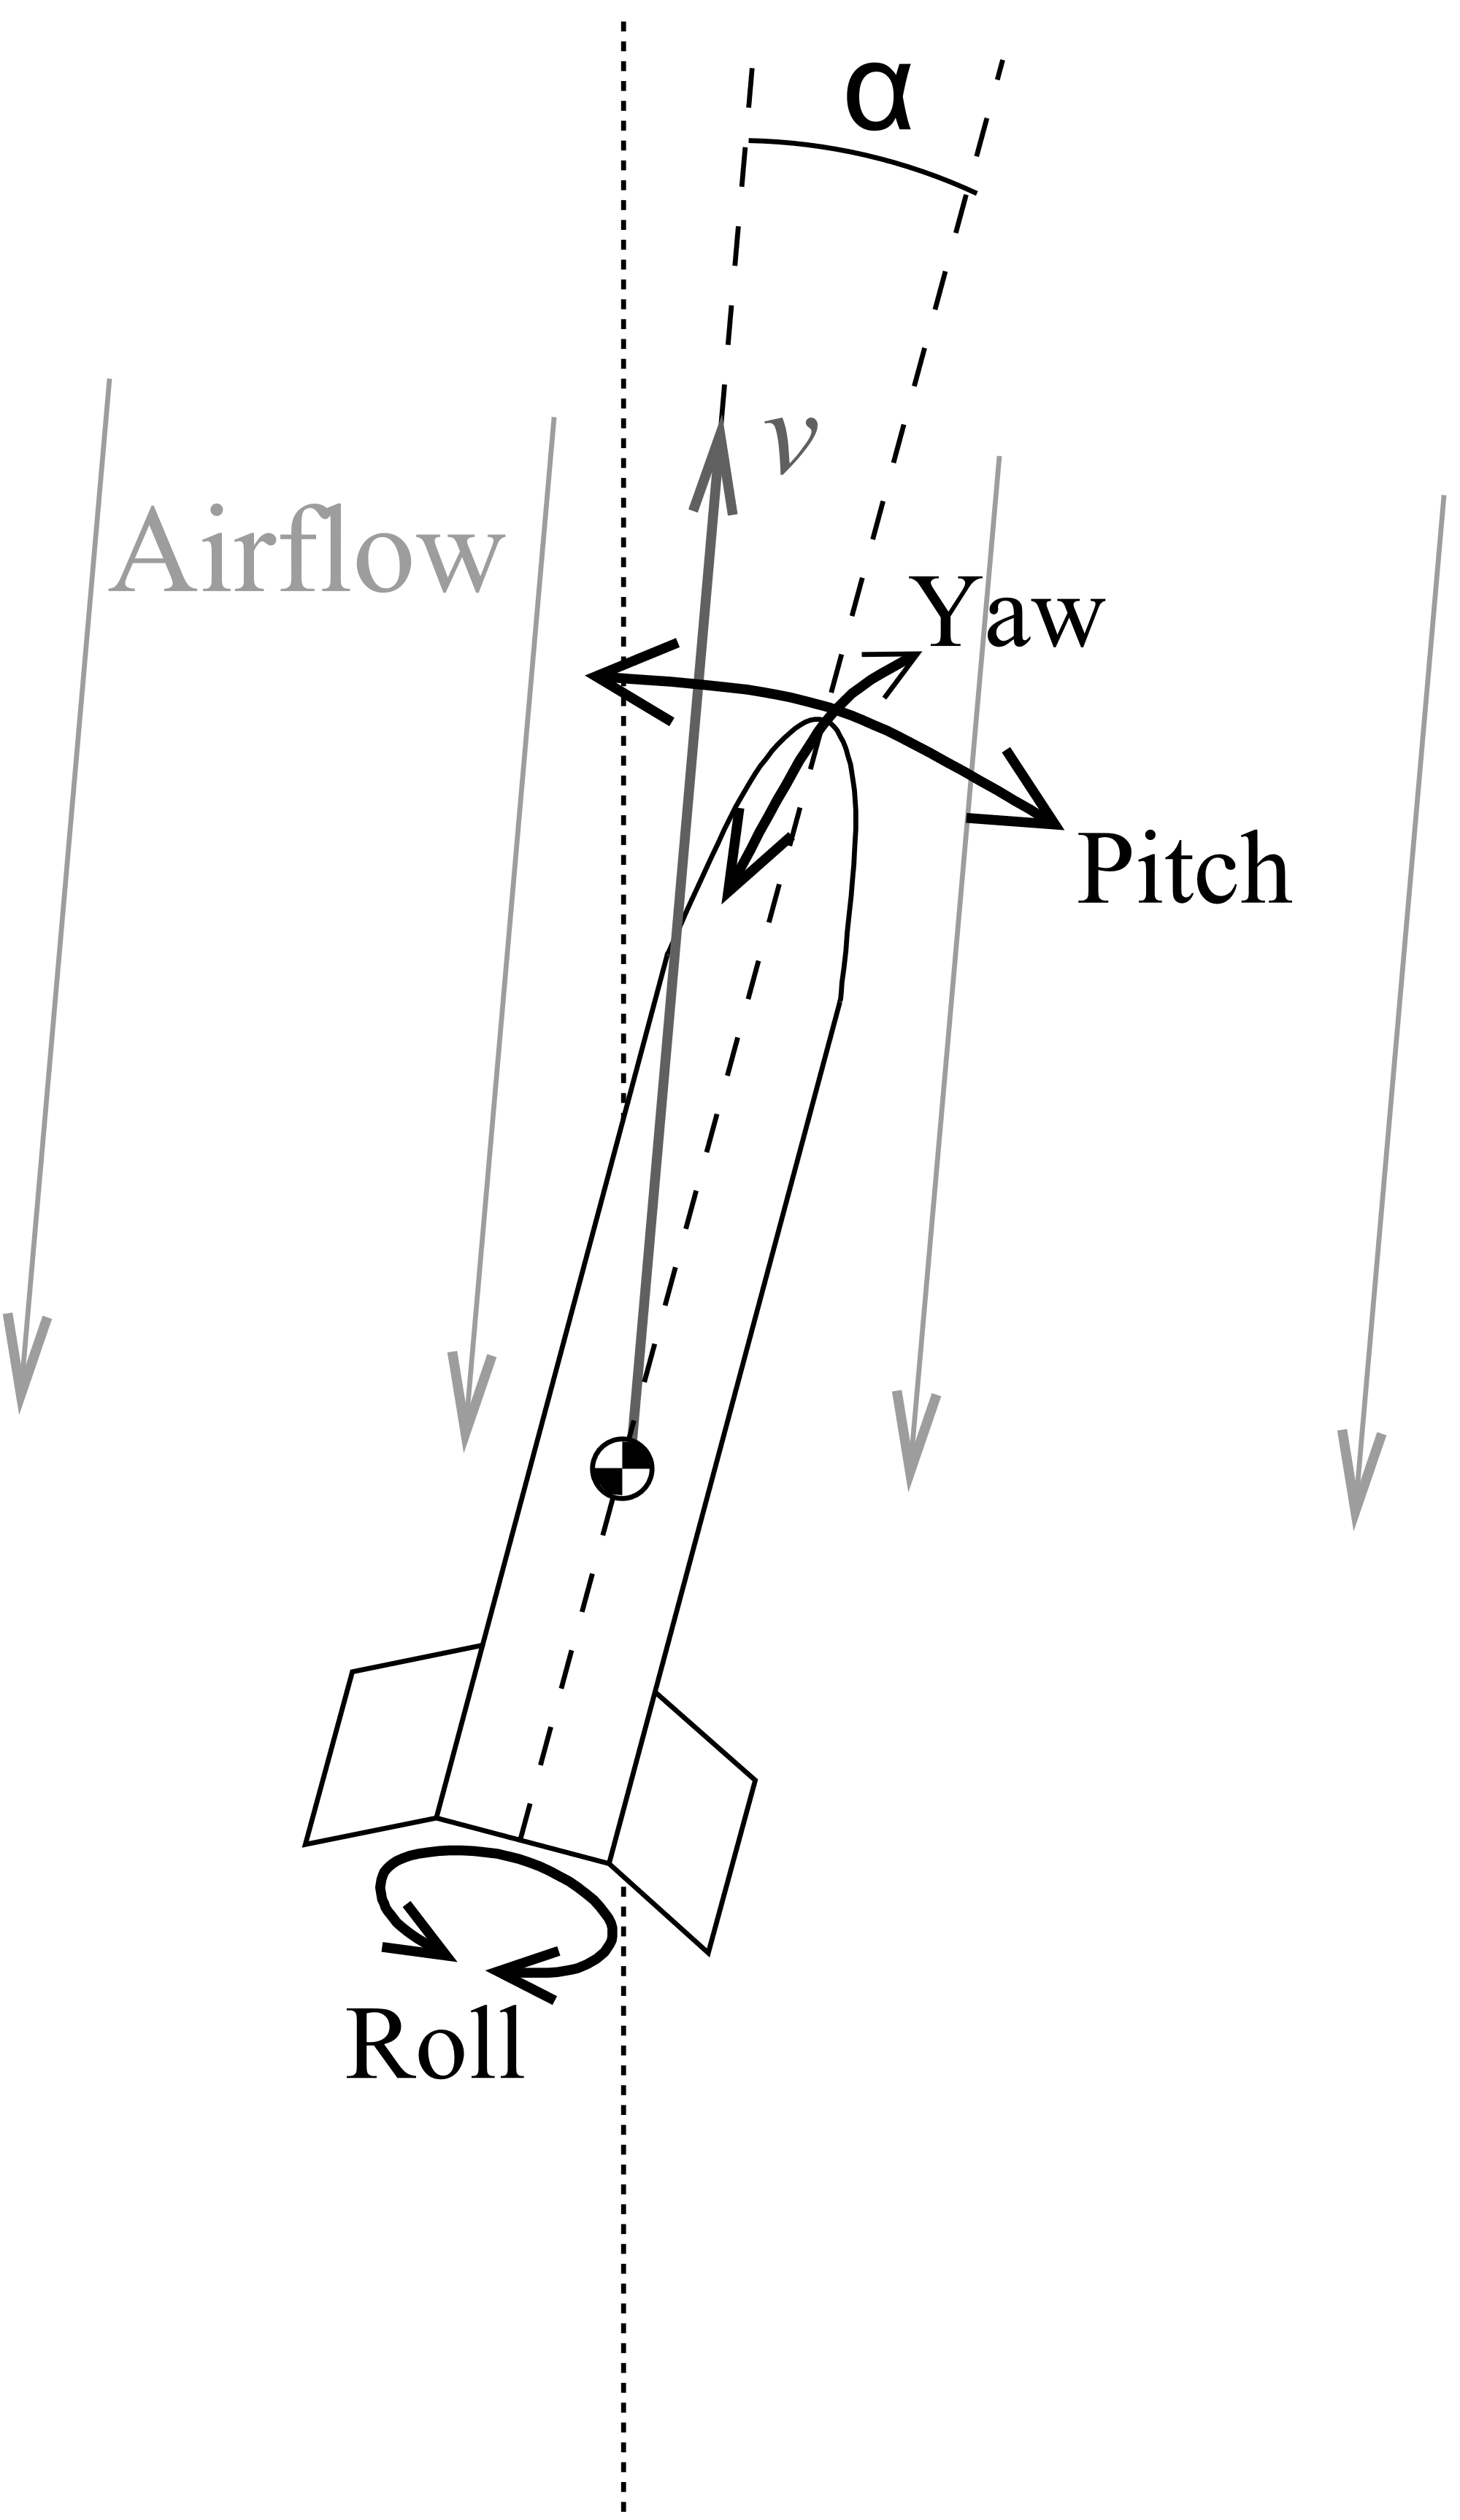
\includegraphics[scale = 0.06, trim={0 15cm 0 0},clip]{Rocket,pitch-yaw-roll}
        \caption{The pitch, yaw and roll directions in the $b$ frame.~\cite{OR}}
    \end{subfigure}
\end{figure}
%
\subsection{Attitude}
The aerodynamic moments acting on the body are as follows, with the coefficients again defined in~\fullrefnocomma{subsec:Coefficients}.
\begin{align}
    \mathbf{AeroMoments}^b &= \frac{1}{2} \rho \norm{\m v_\infty}^2 A_{ref} * d_{ref} * \mathbf{Rot} \begin{bmatrix}
    -C_y \\
    C_m \\
    C_l
    \end{bmatrix}
    \intertext{The net moment is the sum of the aerodynamic moments and the actuator moments from the \gls{tvc} gimbal and the reaction wheel}
    \m{\tau}^b &= \mathbf{AeroMoments}^b + \amom \\
    [\dot{\m \omega^b}]^{bn} &= (\m{I}^b)\inv ( \m{\tau}^b - [\m{\omega}^b]^{bn} \times \m{I}^b [\m{\omega}^b]^{bn} ) \\
    \dot{\q}^{nb} &= \frac{1}{2} \q^{nb}
    \begin{bmatrix}
        0 \\
        [\m{\omega}^b]^{bn}
    \end{bmatrix}
\end{align}